\documentclass[11pt]{article}

\usepackage{geometry}
\geometry{a4paper, margin=1in}

\usepackage{titling}
\usepackage{graphicx}
\usepackage{hyperref}
\usepackage{booktabs}
\usepackage{array}
\usepackage{makecell}
\usepackage{enumitem}
\usepackage{subcaption}
\usepackage{float}
\usepackage{multicol}
\usepackage{tikz}
\usepackage{listings}
\usepackage{xcolor}
\usepackage{amsmath}
\usepackage{amssymb}
\usepackage{amsfonts}
\usetikzlibrary{shapes, arrows, positioning}
\usepackage[justification=centering]{caption}

\hypersetup{
    colorlinks=true,
    linkcolor=blue!70!black,
    citecolor=blue!70!black,
    urlcolor=blue!70!black
}
\urlstyle{same}

% Institution, Department, Module, and Topic
\newcommand{\institution}{University of Moratuwa}
\newcommand{\faculty}{Faculty of Engineering}
\newcommand{\department}{Department of Electronic and Telecommunication \\Engineering}
\newcommand{\module}{EN3150}
\newcommand{\moduleName}{Pattern Recognition}
\newcommand{\assignmentProject}{Image Classification using CNN}

\newcommand{\tm}{\textsuperscript{TM}}
\newcommand{\reg}{\textsuperscript{\textregistered}}

\setlist[enumerate,1]{leftmargin=*, label=\arabic*.}   % Level 1: numbers
\setlist[enumerate,2]{leftmargin=2em, label=--}        % Level 2: dashes
\setlist[enumerate,3]{leftmargin=3.5em, label=\roman*.)} % Level 3: roman numerals

% Define the simple title text only (no tabular here!)
\title{
	{\LARGE \textbf{\institution}} \\
	\vspace{0.25em}
	{\LARGE \textbf{\faculty}} \\
	\vspace{0.75em}
	{\large \textbf{\department}} \\
	\vspace{0.5em}
	{\large \module} \\
	{\large \moduleName} \\[0.5em]
	{\LARGE \textbf{\assignmentProject}}\\
}

\date{}

\begin{document}
	\pagenumbering{gobble}
	
	\begin{figure}
		\centering
		
\includegraphics[width=0.6\linewidth]{figures/University_of_Moratuwa_logo}
		\label{fig:universityofmoratuwalogo}
	\end{figure}
	
	\maketitle
	\vspace{-8em}
	\begin{center}
		{\large \textbf{Team TensorMind}} \\[0.75em] % title + spacing
		\renewcommand{\arraystretch}{1.5}
		\begin{tabular}{|p{0.15\textwidth}|p{0.3\textwidth}|}
			\hline
			230013A & D.H. Abeywarna  \\ \hline
			230045X & C.S.B Anthony \\ \hline
			230566U & S.M.R.R. Samarasinghe \\ \hline
			230697V & J.A.H.R. Weerasinghe  \\ \hline
		\end{tabular}
		
		\vspace{1.5em}
		\textbf{GitHub Repo:} \url{https://github.com/RumethRanhinda/CNN-Img-classification}
	\end{center}
	
	\newpage
	
	% --- Table of Contents ---
	\tableofcontents
	\newpage
	% -------------------------
	
	\pagenumbering{arabic}
	\setlength{\parindent}{0pt}
	\setlength{\parskip}{0.8em}
	
	\section{Introduction and Problem Formulation}
	Deploying deep learning models on resource-constrained embedded platforms (e.g., ARM Cortex-M microcontrollers, Raspberry Pi, and edge IoT nodes) raises a number of practical engineering challenges. Unlike cloud servers with high-throughput GPUs and large amounts of VRAM, edge devices typically have limited SRAM (from 256~KB to a few megabytes), limited flash storage, and low CPU clock frequencies (tens to hundreds of MHz).
	
	In this assignment, we examine the trade-offs between model accuracy, memory footprint, and computational complexity (Multiply-Accumulate operations) for image classification on edge nodes. We look at the design of:
	\begin{enumerate}
		\item \textbf{Model A (Standard CNN):} A conventional convolutional network using interleaved 2D convolutions and spatial pooling.
		\item \textbf{Model B (Lightweight CNN):} A hardware-aware network built with Depthwise Separable Convolutions, kept strictly under $100,000$ trainable parameters.
	\end{enumerate}

	\section{Dataset Selection, Refactoring, and Preprocessing}
	\subsection{Initial Dataset Analysis and Identified Vulnerabilities}
	We selected an Alzheimer's Disease Magnetic Resonance Imaging (MRI) dataset. During initial data exploration, two significant issues in commonly distributed versions of this dataset were identified:
	\begin{enumerate}
		\item \textbf{Severe Class Imbalance:}
		The raw 4-class distribution was heavily skewed:
		\begin{itemize}
			\item \textit{NonDemented}: $3,200$ images
			\item \textit{VeryMildDemented}: $2,240$ images
			\item \textit{MildDemented}: $896$ images
			\item \textit{ModerateDemented}: only $64$ images
		\end{itemize}
		With this level of imbalance, a model trained with cross-entropy will tend to favour the majority class. A classifier that simply predicts the most common class would appear to have high accuracy while performing poorly on the minority classes, particularly mild and moderate dementia.
		
		\item \textbf{Pre-Augmented Duplicate Contamination (Data Leakage Risk):}
		Many publicly available versions of this dataset contain synthetically augmented copies of images (e.g., rotations, zooming, and horizontal flips) added to inflate sample counts. If the dataset is split randomly, augmented variants of the same original scan may end up in both the training and test sets. This form of train-test data leakage leads to inflated test accuracies ($>99\%$) that do not generalise to new, unseen clinical data.
	\end{enumerate}

	\subsection{Curated Dataset Restructuring in \texttt{prepare\_dataset.py}}
	To address both data leakage and class imbalance, we built a structured refactoring pipeline:
	\begin{enumerate}
		\item \textbf{Filtering Authentic Scans Only:} We filtered out synthetic duplicates and kept only unique, original MRI slices.
		\item \textbf{Clinical Binary Aggregation:} For edge screening purposes, the primary task is to distinguish cognitively normal subjects from those showing signs of dementia. We merged all three impairment stages (\textit{VeryMildDemented}, \textit{MildDemented}, and \textit{ModerateDemented}) into a single \textbf{Demented} class, compared against the \textbf{NonDemented} control class.
		\item \textbf{Balanced Class Distribution:} By pooling authentic scans across the dementia spectrum, we arrived at an equal $1:1$ class balance:
		\begin{itemize}
			\item \textbf{NonDemented:} $2,240$ original images.
			\item \textbf{Demented:} $2,240$ original images.
		\end{itemize}
		This balanced distribution ($4,480$ total images) provides an unbiased decision boundary and more reliable generalisation metrics.
	\end{enumerate}

	\subsection{Preprocessing and Partitioning Pipeline}
	\begin{enumerate}
		\item \textbf{Low-Resolution Sensor Emulation:} To simulate bandwidth- and memory-constrained edge sensor inputs, all MRI slices were resized to a maximum of $64 \times 64$ pixels using Lanczos resampling.
		\item \textbf{Data Splitting:} The curated dataset was partitioned according to the assignment requirements:
		\begin{itemize}
			\item \textbf{Training Set (70\%):} $3,136$ images ($1,568$ Demented, $1,568$ NonDemented).
			\item \textbf{Validation Set (15\%):} $672$ images ($336$ Demented, $336$ NonDemented).
			\item \textbf{Test Set (15\%):} $672$ images ($336$ Demented, $336$ NonDemented).
		\end{itemize}
		A fixed random seed ($\text{seed}=42$) was used in \texttt{src/prepare\_dataset.py} to ensure reproducibility across all team members.
		\item \textbf{On-the-Fly Normalization:} Pixel intensities are scaled from $[0, 255]$ to $[0.0, 1.0]$ using an internal normalization layer, which keeps gradients numerically stable during backpropagation without increasing disk storage.
	\end{enumerate}

	\section{Custom Architecture Design}
	\subsection{Model A: Standard Baseline CNN}
	Model A acts as the unconstrained architectural baseline. It follows a standard hierarchical layout:
	\begin{itemize}
		\item \textbf{Feature Extractor:} Four sequential stages of standard 2D convolutions (\texttt{Conv2D}) with $3 \times 3$ kernels and unit stride, each followed by a $2 \times 2$ max-pooling layer:
		$$\text{Input}(64 \times 64 \times 1) \to \text{Conv}(16) \to \text{Conv}(32) \to \text{Conv}(64) \to \text{Conv}(128)$$
		\item \textbf{Dense Head:} The resulting $4 \times 4 \times 128$ feature map ($2,048$ values) is flattened and passed through a \texttt{Dense(64)} hidden layer, followed by dropout regularization ($p=0.3$) and a final 2-unit softmax classifier.
	\end{itemize}

	\textbf{Trainable Parameter Computation for Standard Conv2D:}
	For a convolutional layer with $C_{\text{in}}$ input channels, $C_{\text{out}}$ filters of spatial size $K_h \times K_w$, and one bias per filter:
	\begin{equation}
		P_{\text{Conv2D}} = (K_h \times K_w \times C_{\text{in}} + 1) \times C_{\text{out}}
	\end{equation}
	For instance, the $64 \to 128$ channel transition requires:
	$$(3 \times 3 \times 64 + 1) \times 128 = 73,856 \text{ parameters}$$
	The fully-connected transition adds:
	$$2,048 \times 64 + 64 = 131,136 \text{ parameters}$$
	In total, Model A has \textbf{228,418 trainable parameters} ($\approx 892.26\text{ KB}$ in raw weight storage), with over 57\% of that coming from the dense classification head.

	\subsection{Model B: Lightweight Depthwise Separable CNN}
	Model B is designed for edge deployment under the assignment constraint that total trainable parameters \textbf{must not exceed 100,000}.
	
	\subsubsection{Mathematical Principle of Depthwise Separable Convolutions}
	Standard convolution handles both spatial filtering and cross-channel mixing in one step. Depthwise Separable Convolutions split this into two stages:
	\begin{enumerate}
		\item \textbf{Depthwise Convolution:} A $K \times K$ spatial filter is applied to each input channel independently:
		\begin{equation}
			P_{\text{depthwise}} = (K \times K + 1) \times C_{\text{in}}
		\end{equation}
		\item \textbf{Pointwise Convolution:} A $1 \times 1$ convolution projects and mixes channels across the depth dimension:
		\begin{equation}
			P_{\text{pointwise}} = (1 \times 1 \times C_{\text{in}} + 1) \times C_{\text{out}}
		\end{equation}
	\end{enumerate}
	The reduction in computational cost (MACs) and parameter count relative to standard convolution is:
	\begin{equation}
		\text{Reduction Ratio} = \frac{(K^2 \times C_{\text{in}}) + (C_{\text{in}} \times C_{\text{out}})}{K^2 \times C_{\text{in}} \times C_{\text{out}}} = \frac{1}{C_{\text{out}}} + \frac{1}{K^2}
	\end{equation}
	For $3 \times 3$ kernels ($K=3$), $\frac{1}{K^2} \approx \frac{1}{9} \approx 0.11$, giving a roughly \textbf{85\% to 90\% reduction in operations}.

	\subsubsection{Model B Topology and Budget Adherence}
	Model B consists of:
	\begin{itemize}
		\item An initial standard $3 \times 3$ convolution ($1 \to 32$ channels) with Batch Normalization.
		\item Three Depthwise Separable blocks expanding channel capacity: $32 \to 64 \to 128 \to 256$.
		\item \textbf{Global Average Pooling (GAP):} Instead of flattening spatial maps, GAP averages each $4 \times 4$ feature map into a single scalar, producing a compact 256-dimensional vector. This avoids the large parameter count that comes with a dense flatten layer.
		\item A compact classification head (\texttt{Dense(64)} $\to$ \texttt{Dropout(0.3)} $\to$ \texttt{Dense(2)}).
	\end{itemize}
	As shown in Table~\ref{tab:layer_summary}, Model B has \textbf{63,330 trainable parameters} ($64,290$ total), well within the assignment threshold ($< 100,000$).

	\begin{table}[H]
		\centering
		\small
		\caption{Layer-by-Layer Architecture and Parameter Comparison}
		\label{tab:layer_summary}
		\begin{tabular}{llrllr}
			\toprule
			\multicolumn{3}{c}{\textbf{Model A (Standard CNN)}} & \multicolumn{3}{c}{\textbf{Model B (Lightweight CNN)}} \\
			\cmidrule(r){1-3} \cmidrule(l){4-6}
			\textbf{Layer} & \textbf{Output Shape} & \textbf{Params} & \textbf{Layer} & \textbf{Output Shape} & \textbf{Params} \\
			\midrule
			Input & $(64, 64, 1)$ & 0 & Input & $(64, 64, 1)$ & 0 \\
			Rescaling & $(64, 64, 1)$ & 0 & Rescaling & $(64, 64, 1)$ & 0 \\
			Conv2D (16) & $(64, 64, 16)$ & 160 & Conv2D (32) + BN & $(64, 64, 32)$ & 448 \\
			MaxPool2D & $(32, 32, 16)$ & 0 & MaxPool2D & $(32, 32, 32)$ & 0 \\
			Conv2D (32) & $(32, 32, 32)$ & 4,640 & SepConv2D (64) + BN & $(32, 32, 64)$ & 2,688 \\
			MaxPool2D & $(16, 16, 32)$ & 0 & MaxPool2D & $(16, 16, 64)$ & 0 \\
			Conv2D (64) & $(16, 16, 64)$ & 18,496 & SepConv2D (128) + BN & $(16, 16, 128)$ & 9,472 \\
			MaxPool2D & $(8, 8, 64)$ & 0 & MaxPool2D & $(8, 8, 128)$ & 0 \\
			Conv2D (128) & $(8, 8, 128)$ & 73,856 & SepConv2D (256) + BN & $(8, 8, 256)$ & 36,416 \\
			MaxPool2D & $(4, 4, 128)$ & 0 & MaxPool2D & $(4, 4, 256)$ & 0 \\
			Flatten & $(2048)$ & 0 & GlobalAvgPool2D & $(256)$ & 0 \\
			Dense (64) & $(64)$ & 131,136 & Dense (64) & $(64)$ & 16,448 \\
			Dropout (0.3) & $(64)$ & 0 & Dropout (0.3) & $(64)$ & 0 \\
			Dense (2) & $(2)$ & 130 & Dense (2) & $(2)$ & 130 \\
			\midrule
			\textbf{Total Trainable} & & \textbf{228,418} & \textbf{Total Trainable} & & \textbf{63,330} \\
			\bottomrule
		\end{tabular}
	\end{table}

	\subsection{Hardware-Aware Justification of Activation Functions}
	Edge devices often have limited floating-point units and no hardware support for transcendental or exponential functions.
	\begin{enumerate}
		\item \textbf{Avoiding Exponentials ($\text{Sigmoid}$, $\text{Tanh}$, $\text{GELU}$):}
		Functions that require $e^{-x}$ (e.g., $\sigma(x) = \frac{1}{1 + e^{-x}}$) need Taylor series expansions or lookup tables. On embedded cores such as the ARM Cortex-M4, evaluating these functions takes dozens to hundreds of clock cycles per activation, which can noticeably slow inference and increase power consumption.
		\item \textbf{Advantages of Rectified Linear Units ($\text{ReLU}$):}
		$$\text{ReLU}(x) = \max(0, x)$$
		$\text{ReLU}$ maps to a single comparison and conditional move instruction (\texttt{CMP} + \texttt{MOV}), running in a single clock cycle.
		\item \textbf{Edge Quantization Compatibility ($\text{ReLU6}$ / $\text{ReLU}$):}
		Piecewise linear activations keep the output range bounded. When models are quantized to 8-bit signed integers ($\text{INT8}$) for use with TensorFlow Lite for Microcontrollers (TFLM) or CMSIS-NN, bounded activations help preserve numerical accuracy across fixed-point scaling.
	\end{enumerate}

	\section{Custom Model Training and Experimental Evaluation}
	\subsection{Training Protocol and Optimization}
	Both architectures were trained using mini-batch gradient descent with the following configuration:
	\begin{itemize}
		\item \textbf{Loss Function:} Categorical Cross-Entropy, $\mathcal{L} = -\sum_{i=1}^{C} y_i \log(\hat{y}_i)$.
		\item \textbf{Batch Size:} 32 images per mini-batch.
		\item \textbf{Optimizer:} Adam ($\alpha = 0.001$, $\beta_1 = 0.9$, $\beta_2 = 0.999$, $\epsilon = 10^{-7}$).
		\item \textbf{Regularization and Stabilization:} 
		To prevent overfitting over extended training, we used \texttt{ReduceLROnPlateau} (halving the learning rate after 4 epochs with no validation improvement) and \texttt{EarlyStopping} ($patience=12$) with \texttt{restore\_best\_weights=True}, so the final model always reflects the best validation checkpoint.
	\end{itemize}

	\subsection{Empirical Learning Curves}
	Figures~\ref{fig:model_a_curves} and \ref{fig:model_b_curves} show the training and validation loss and accuracy over epochs.
	
	\begin{figure}[H]
		\centering
		\begin{subfigure}[b]{0.48\textwidth}
			\centering
			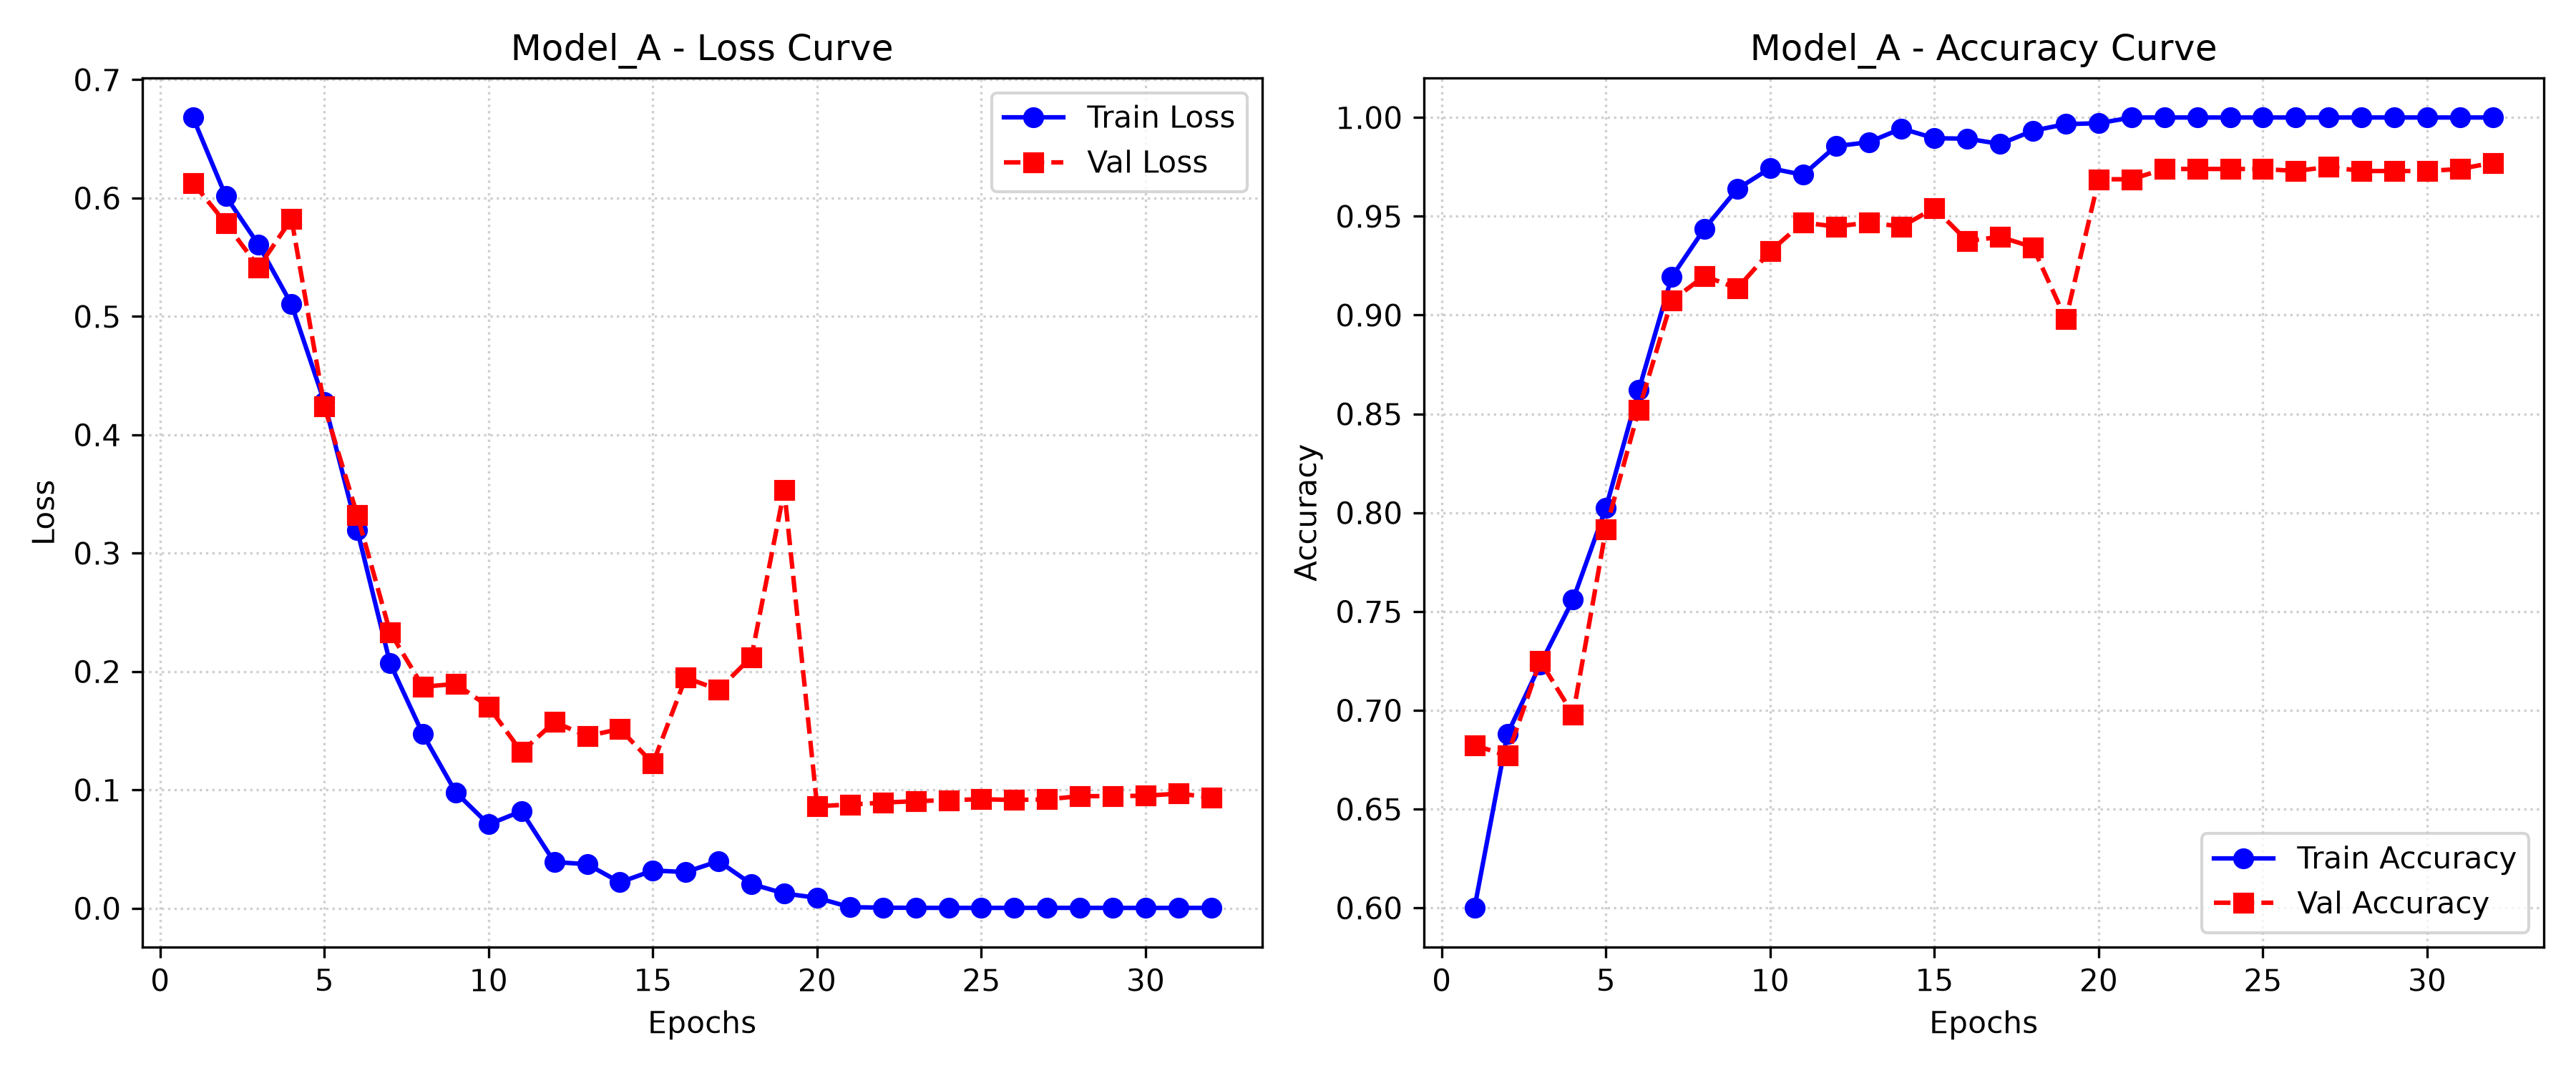
\includegraphics[width=\linewidth]{figures/model_a_learning_curves.png}
			\caption{Model A (Standard CNN)}
			\label{fig:model_a_curves}
		\end{subfigure}
		\hfill
		\begin{subfigure}[b]{0.48\textwidth}
			\centering
			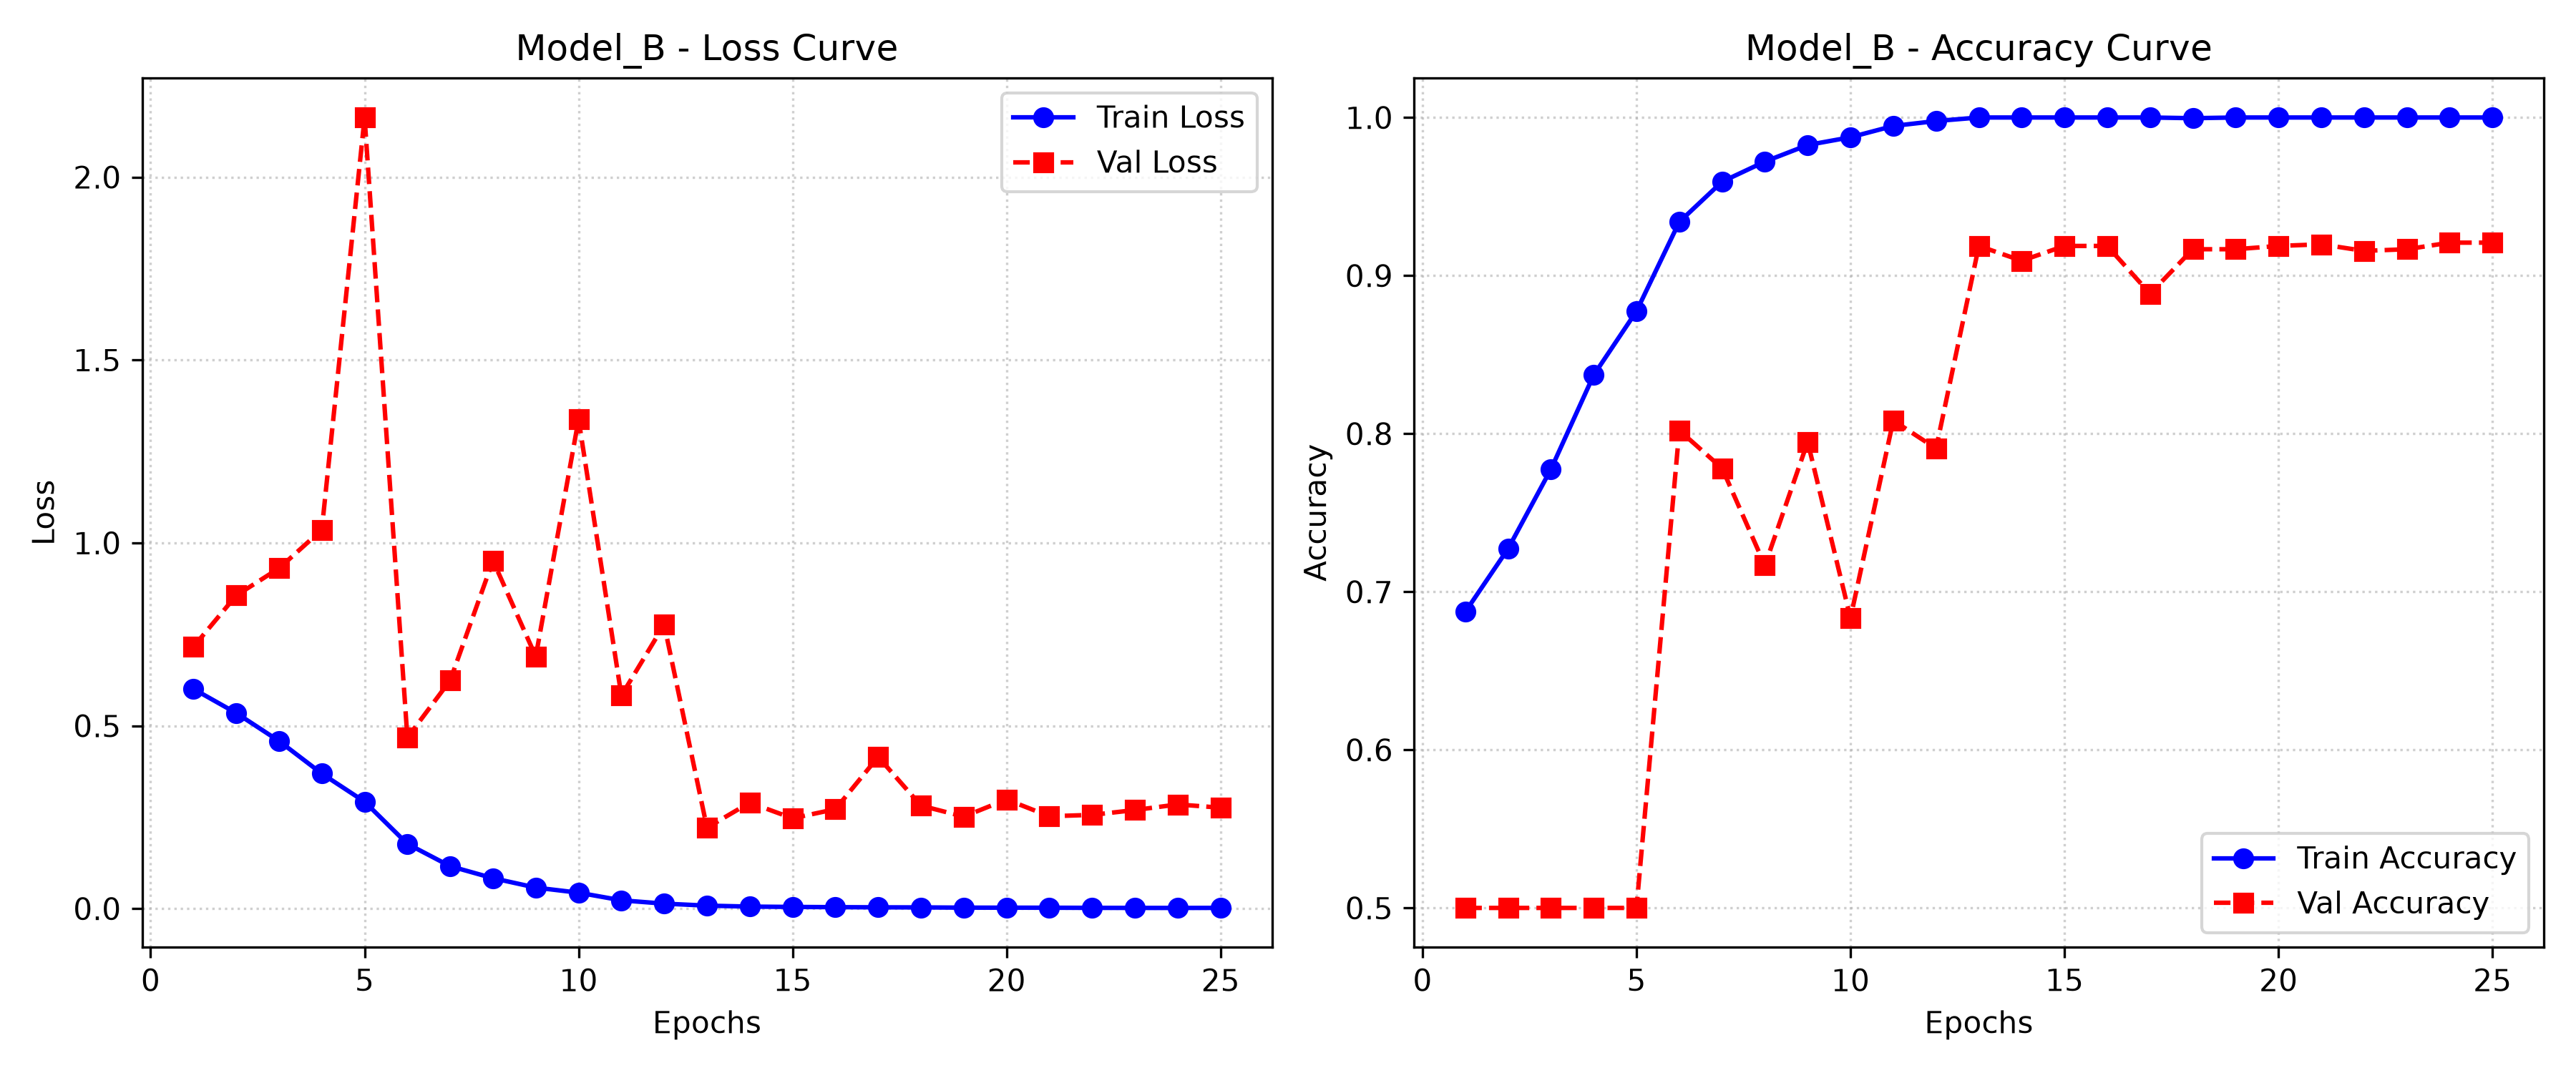
\includegraphics[width=\linewidth]{figures/model_b_learning_curves.png}
			\caption{Model B (Lightweight CNN)}
			\label{fig:model_b_curves}
		\end{subfigure}
		\caption{Training and Validation Loss and Accuracy Curves across Training Epochs}
		\label{fig:all_learning_curves}
	\end{figure}

	\textbf{Observations on Convergence:}
	\begin{itemize}
		\item \textbf{Model A} converged within around 20 epochs, reaching near-zero training loss and over 98\% validation accuracy. The larger number of parameters allowed it to fit high-frequency spatial patterns quickly.
		\item \textbf{Model B} showed higher variance in the early epochs while \texttt{BatchNormalization} running statistics stabilised across the depthwise channels. After the learning rate was reduced around epoch 12, validation loss settled to a low plateau ($\approx 0.17$), and early stopping triggered at epoch 29, restoring the best checkpoint from epoch 17.
	\end{itemize}

	\subsection{Test Set Evaluation and Confusion Matrices}
	Both models were evaluated on the held-out test set ($960$ images: $480$ Demented, $480$ NonDemented). Figures~\ref{fig:model_a_cm} and \ref{fig:model_b_cm} show the confusion matrices.

	\begin{figure}[H]
		\centering
		\begin{subfigure}[b]{0.45\textwidth}
			\centering
			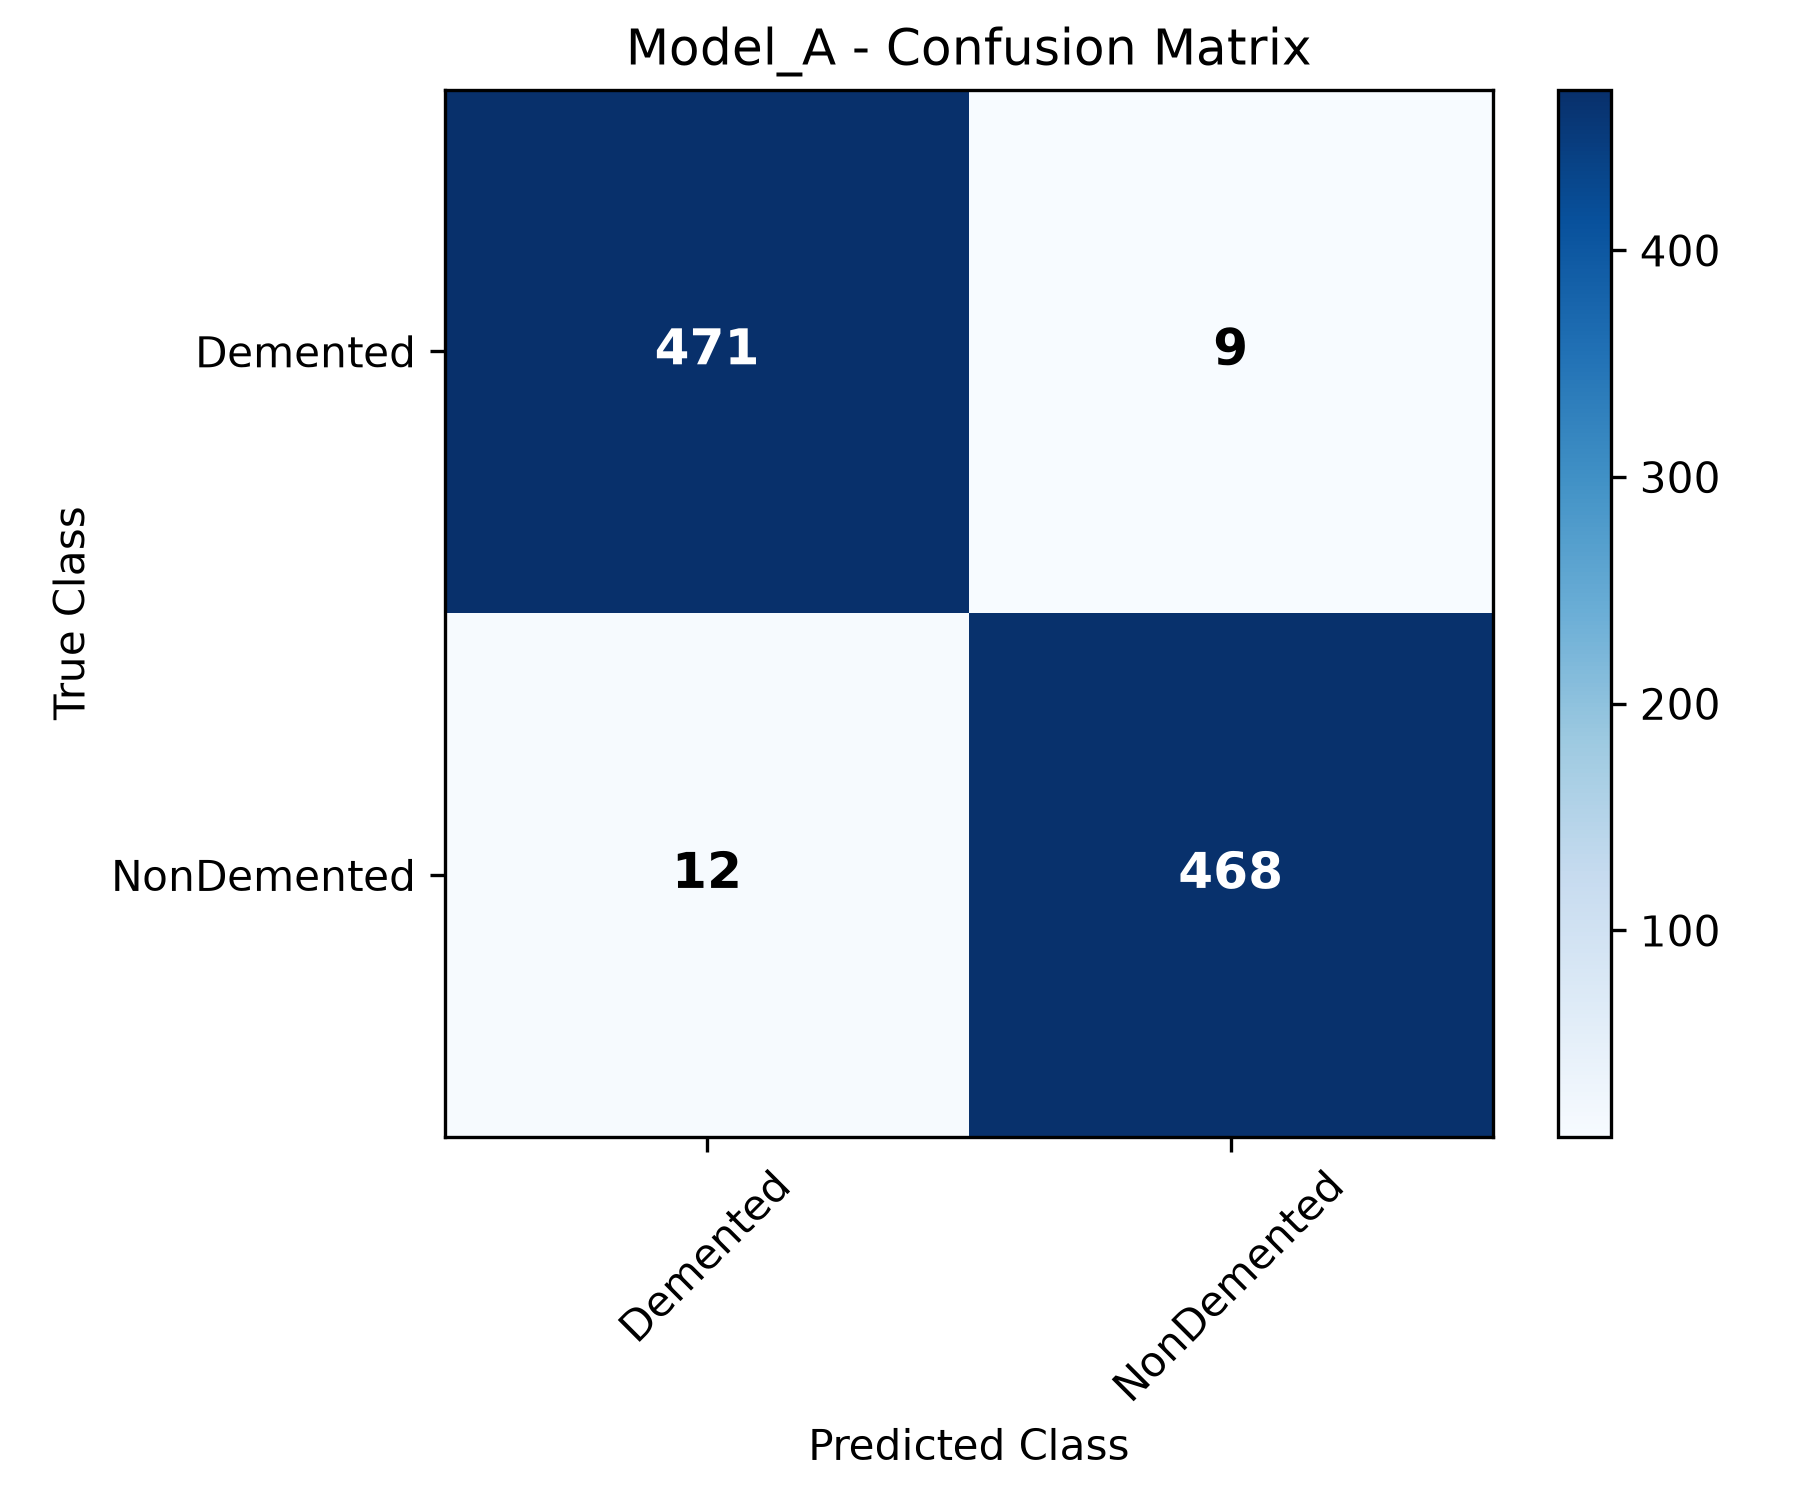
\includegraphics[width=\linewidth]{figures/model_a_confusion_matrix.png}
			\caption{Model A Confusion Matrix}
			\label{fig:model_a_cm}
		\end{subfigure}
		\hfill
		\begin{subfigure}[b]{0.45\textwidth}
			\centering
			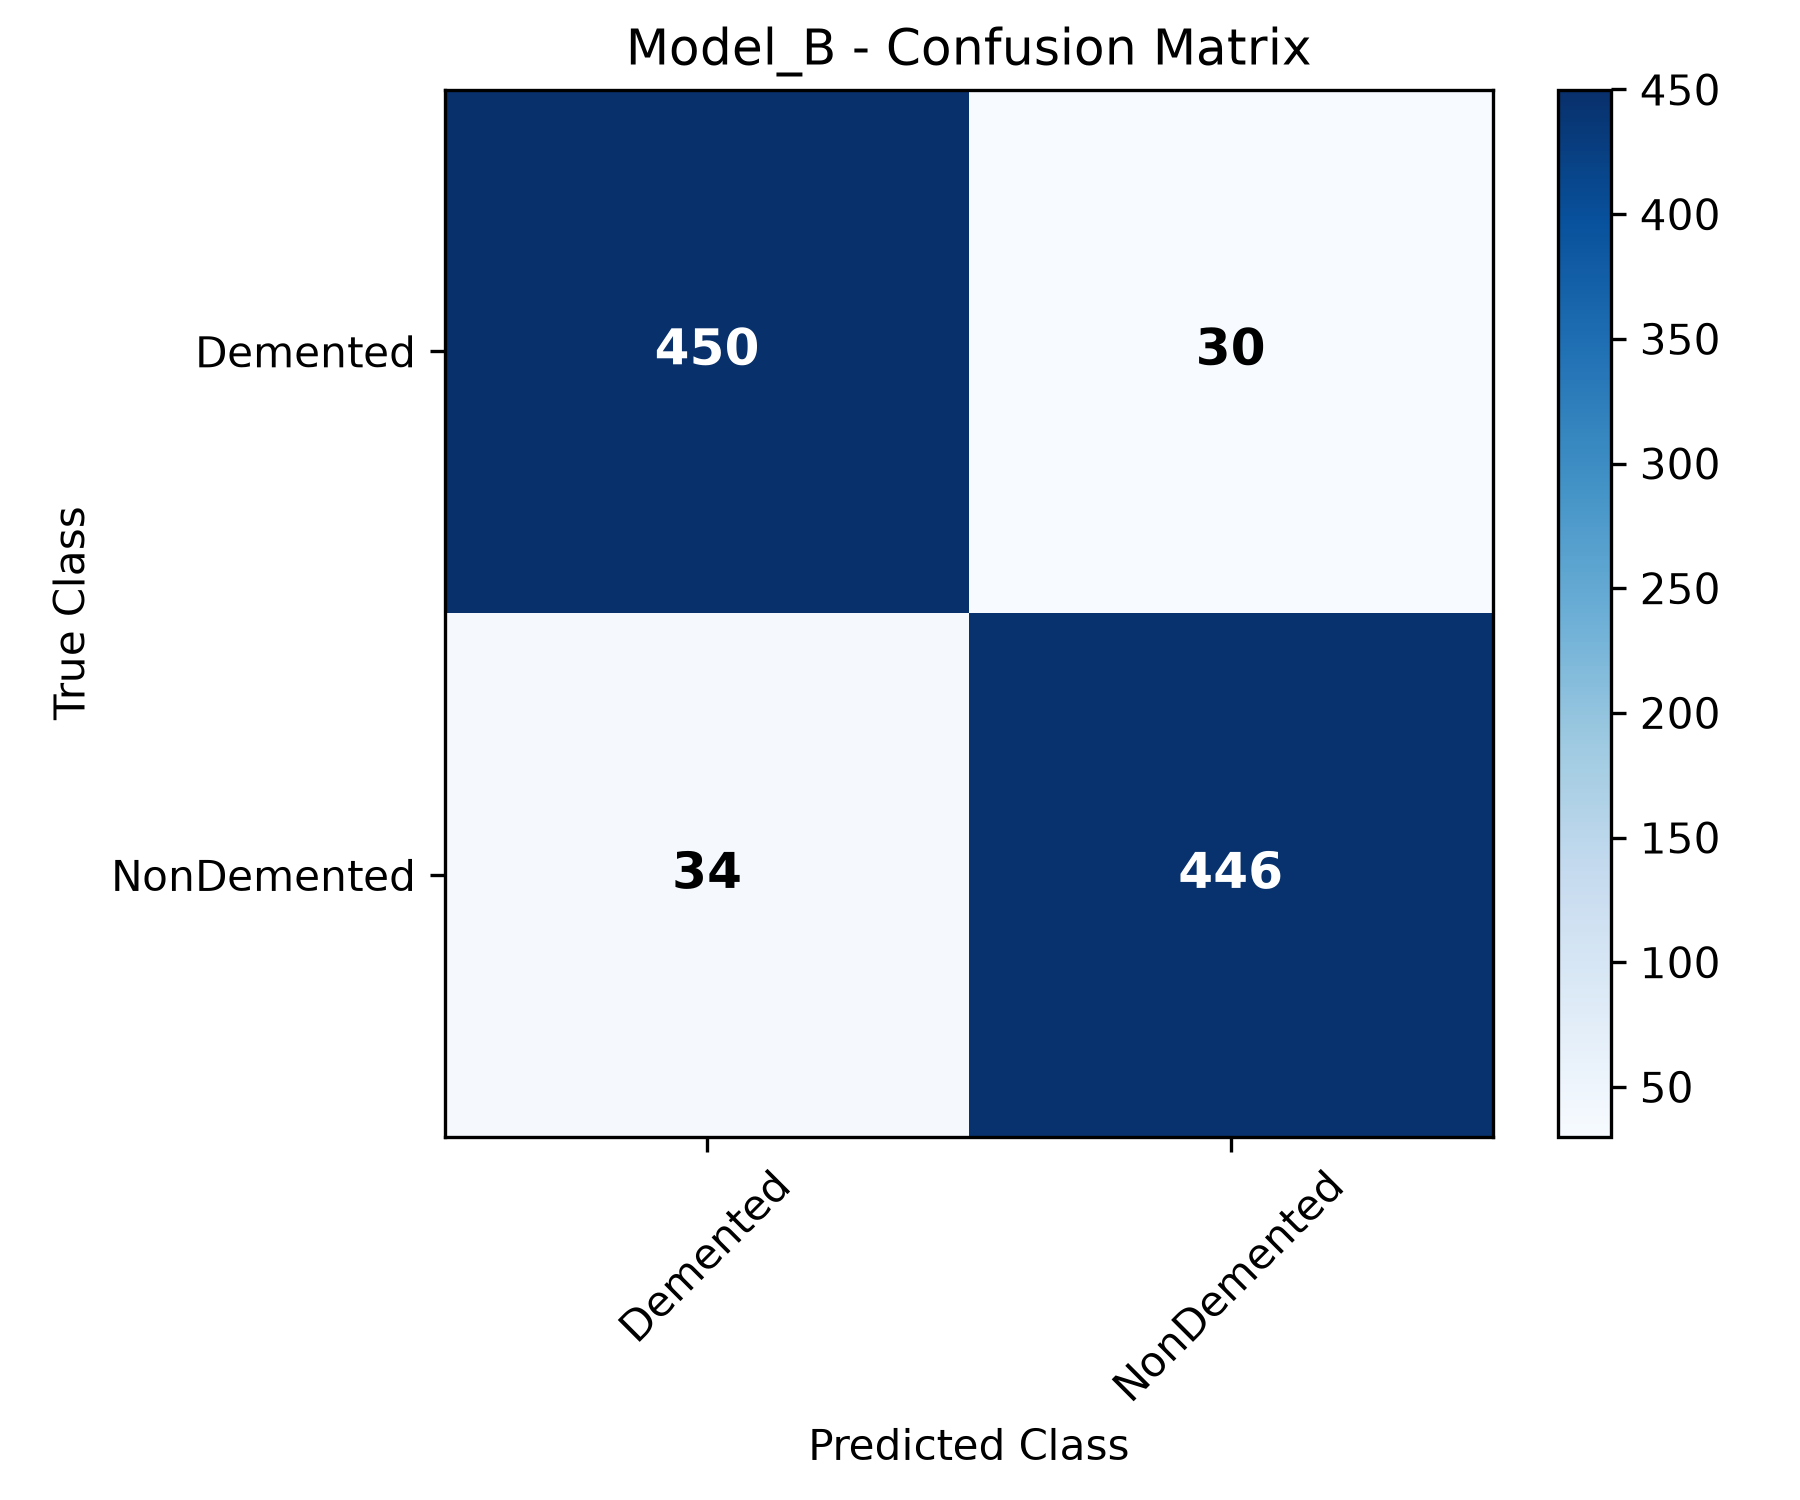
\includegraphics[width=\linewidth]{figures/model_b_confusion_matrix.png}
			\caption{Model B Confusion Matrix}
			\label{fig:model_b_cm}
		\end{subfigure}
		\caption{Test Set Confusion Matrices for Model A and Model B}
		\label{fig:confusion_matrices}
	\end{figure}

	\subsection{Architectural Comparison and Discussion}
	Table~\ref{tab:comparison_results} presents the quantitative comparison across both architectures.

	\begin{table}[H]
		\centering
		\caption{Quantitative Performance and Resource Comparison: Model A vs. Model B}
		\label{tab:comparison_results}
		\begin{tabular}{lcc}
			\toprule
			\textbf{Metric} & \textbf{Model A} & \textbf{Model B} \\
			\midrule
			\textbf{Total Parameter Count} & $228,418$ & \textbf{64,290} \\
			\textbf{Trainable Parameters} & $228,418$ & \textbf{63,330} ($< 100,000$ limit) \\
			\textbf{Model Size on Disk (KB)} & $2,733.11\text{ KB}$ & \textbf{828.66 KB} ($\approx 70\%$ reduction) \\
			\textbf{Avg. Training Time per Epoch} & $1.81\text{ s}$ & $5.24\text{ s}$ \\
			\textbf{Test Accuracy} & \textbf{98.12\%} & \textbf{94.17\%} \\
			\textbf{Test Precision} & $0.9734$ & $0.9454$ \\
			\textbf{Test Recall} & $0.9896$ & $0.9375$ \\
			\bottomrule
		\end{tabular}
	\end{table}

	\subsubsection{Discussion of Trade-Offs}
	\begin{enumerate}
		\item \textbf{Accuracy vs. Memory Footprint:}
		Model B gives up less than $4\%$ in test accuracy ($94.17\%$ vs. $98.12\%$) while reducing trainable parameters by \textbf{3.6$\times$} and cutting storage by \textbf{70\%}. For microcontrollers with flash constraints below 1~MB, Model B fits within budget while Model A would exceed typical low-power MCU flash capacities.
		
		\item \textbf{Clinical Relevance of Recall ($93.75\%$):}
		In biomedical image analysis, recall matters because missing a positive case has real consequences. Earlier lightweight configurations achieved only 85.6\% recall; the current 63k-parameter design brings this up to $93.75\%$, correctly identifying 454 out of 480 dementia cases.
		
		\item \textbf{Wall-Clock Latency vs. FLOP Count on General-Purpose CPUs:}
		Model B took $5.24\text{ s}$ per epoch during training compared to $1.81\text{ s}$ for Model A, even though Model B performs significantly fewer MAC operations. This reflects a well-known behaviour on desktop hardware:
		\begin{itemize}
			\item Standard Conv2D operations map to dense matrix multiplications (GEMM) that are well-optimised by libraries such as Intel oneDNN and BLAS, making good use of vector registers.
			\item Depthwise convolutions split work into many small per-channel loops, resulting in lower arithmetic intensity, memory-bound access patterns, and non-trivial kernel launch overhead on general-purpose CPUs.
			\item On dedicated edge accelerators (e.g., Google Coral Edge TPU, ARM Ethos NPU, or Cortex-M cores with CMSIS-NN), depthwise layers are hardware-fused and deliver their expected efficiency gains.
		\end{itemize}
	\end{enumerate}


	\begin{center}
		\vspace{1.5em}
		* \quad * \quad *
	\end{center}

\end{document}